\documentclass[tikz]{standalone}
\usepackage{tikz}
\usetikzlibrary{positioning, graphs}
\usetikzlibrary{graphs.standard}
\begin{document}
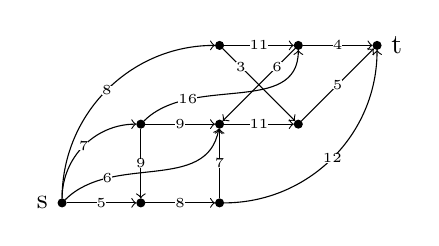
\begin{tikzpicture}
		[vertex/.style={draw,circle,inner sep = 0mm, minimum size = 1mm, fill = black},
		 edgelabel/.style = {fill = white, inner sep = 0mm, font=\tiny}]
		\node[vertex, label=left:s] (s) at (0,0) {};
		\node[vertex] (a) at (1,0) {}
			edge [<-]	node[edgelabel] {$5$}	(s);
		\node[vertex] (b) at (2,0) {}
			edge [<-]	node[edgelabel] {$8$}	(a);
		\node[vertex] (c) at (1,1) {}
			edge [<-, in = 90, out = 180]	node[edgelabel] {$7$}	(s)
			edge [->]	node[edgelabel] {$9$}	(a);
		\node[vertex] (d) at (2,1) {}
			edge [<-, in = 45, out = -100]	node[near end, edgelabel] {$6$}	(s)
			edge [<-]	node[edgelabel] {$9$}	(c)
			edge [<-]	node[edgelabel] {$7$}	(b);
		\node[vertex] (e) at (3,1) {}
			edge [<-]	node[edgelabel] {$11$}	(d);
		\node[vertex] (f) at (2,2) {}
			edge [<-, in = 90, out = 180]	node[edgelabel] {$8$}	(s)
			edge [->]	node[near start, edgelabel] {$3$}	(e);
		\node[vertex] (g) at (3,2) {}
			edge [<-]	node[edgelabel] {$11$}	(f)
			edge [->]	node[near start, edgelabel] {$6$}	(d)
			edge [<-, out = -90, in = 45]	node[near end, edgelabel] {$16$}	(c);
		\node[vertex, label=right:t] (t) at (4,2) {}
			edge [<-]	node[edgelabel] {$4$}	(g)
			edge [<-]	node[edgelabel] {$5$}	(e)
			edge [<-, out = -90, in = 0]	node[edgelabel] {$12$}	(b);
\end{tikzpicture}
\end{document}